% ============================================================
%  CV — Miguel Carranza  (español)
%  Compilar:  tectonic cv.tex      (o xelatex cv.tex)
%  Genera:    cv.pdf  → se publica como Miguel_Carranza_CV.pdf
% ============================================================
\documentclass[10pt]{article}

\usepackage[a4paper, top=0pt, bottom=0pt, left=0pt, right=0pt]{geometry}
\usepackage{fontspec}
\usepackage[default]{sourcesanspro}
\usepackage{xcolor}
\usepackage{tikz}
\usepackage{eso-pic}
\usepackage{fontawesome5}
\usepackage{enumitem}
\usepackage[hidelinks]{hyperref}
\usepackage{microtype}

% ── Colores ──
\definecolor{ink}{HTML}{0A0A0A}
\definecolor{body}{HTML}{3A3A3C}
\definecolor{muted}{HTML}{6E6E73}
\definecolor{accent}{HTML}{0071E3}
\definecolor{side}{HTML}{F2F2F5}
\definecolor{rule}{HTML}{D2D2D7}

\pagestyle{empty}
\setlength{\parindent}{0pt}
\setlength{\parskip}{0pt}
\color{body}

% Barra lateral gris de toda la página
\AddToShipoutPictureBG{%
  \AtPageLowerLeft{\color{side}\rule{0.335\paperwidth}{\paperheight}}}

% ── Comandos de formato ──
\newcommand{\sidetitle}[1]{%
  \vspace{9pt}{\color{ink}\fontsize{8.5}{10}\selectfont\bfseries\addfontfeature{LetterSpace=12}\MakeUppercase{#1}}\par
  \vspace{2pt}{\color{rule}\rule{\linewidth}{0.6pt}}\par\vspace{4pt}}

\newcommand{\maintitle}[1]{%
  \vspace{8pt}{\color{ink}\fontsize{10}{12}\selectfont\bfseries\addfontfeature{LetterSpace=10}\MakeUppercase{#1}}%
  \hspace{6pt}{\color{rule}\leaders\hrule height 3.2pt depth -2.6pt\hfill}\par\vspace{4pt}}

% Puesto: título, lugar, fecha
\newcommand{\job}[3]{%
  {\color{ink}\bfseries\fontsize{10}{12}\selectfont #1}\hfill{\color{muted}\fontsize{8.5}{10}\selectfont #3}\par
  {\color{accent}\fontsize{9}{11}\selectfont #2}\par\vspace{2pt}}

\newcommand{\contact}[2]{\makebox[13pt][l]{\color{accent}\small #1}{\fontsize{8.5}{11}\selectfont #2}\par\vspace{2.5pt}}

\newcommand{\skillgroup}[2]{%
  {\color{ink}\bfseries\fontsize{8.5}{10}\selectfont #1}\par
  {\fontsize{8.5}{11}\selectfont #2}\par\vspace{5pt}}

\setlist[itemize]{leftmargin=10pt, itemsep=0.8pt, topsep=1pt, parsep=0pt,
  label={\color{accent}\scriptsize\textbullet}}

\begin{document}
\fontsize{8.9}{11.6}\selectfont

\noindent
% ============================================================
%  BARRA LATERAL
% ============================================================
\hspace*{20pt}%
\begin{minipage}[t][0.97\paperheight][t]{\dimexpr0.335\paperwidth-38pt\relax}
\vspace{26pt}

% Foto
\begin{center}
\begin{tikzpicture}
  \clip (0,0) circle (1.4cm);
  \node at (0,0) {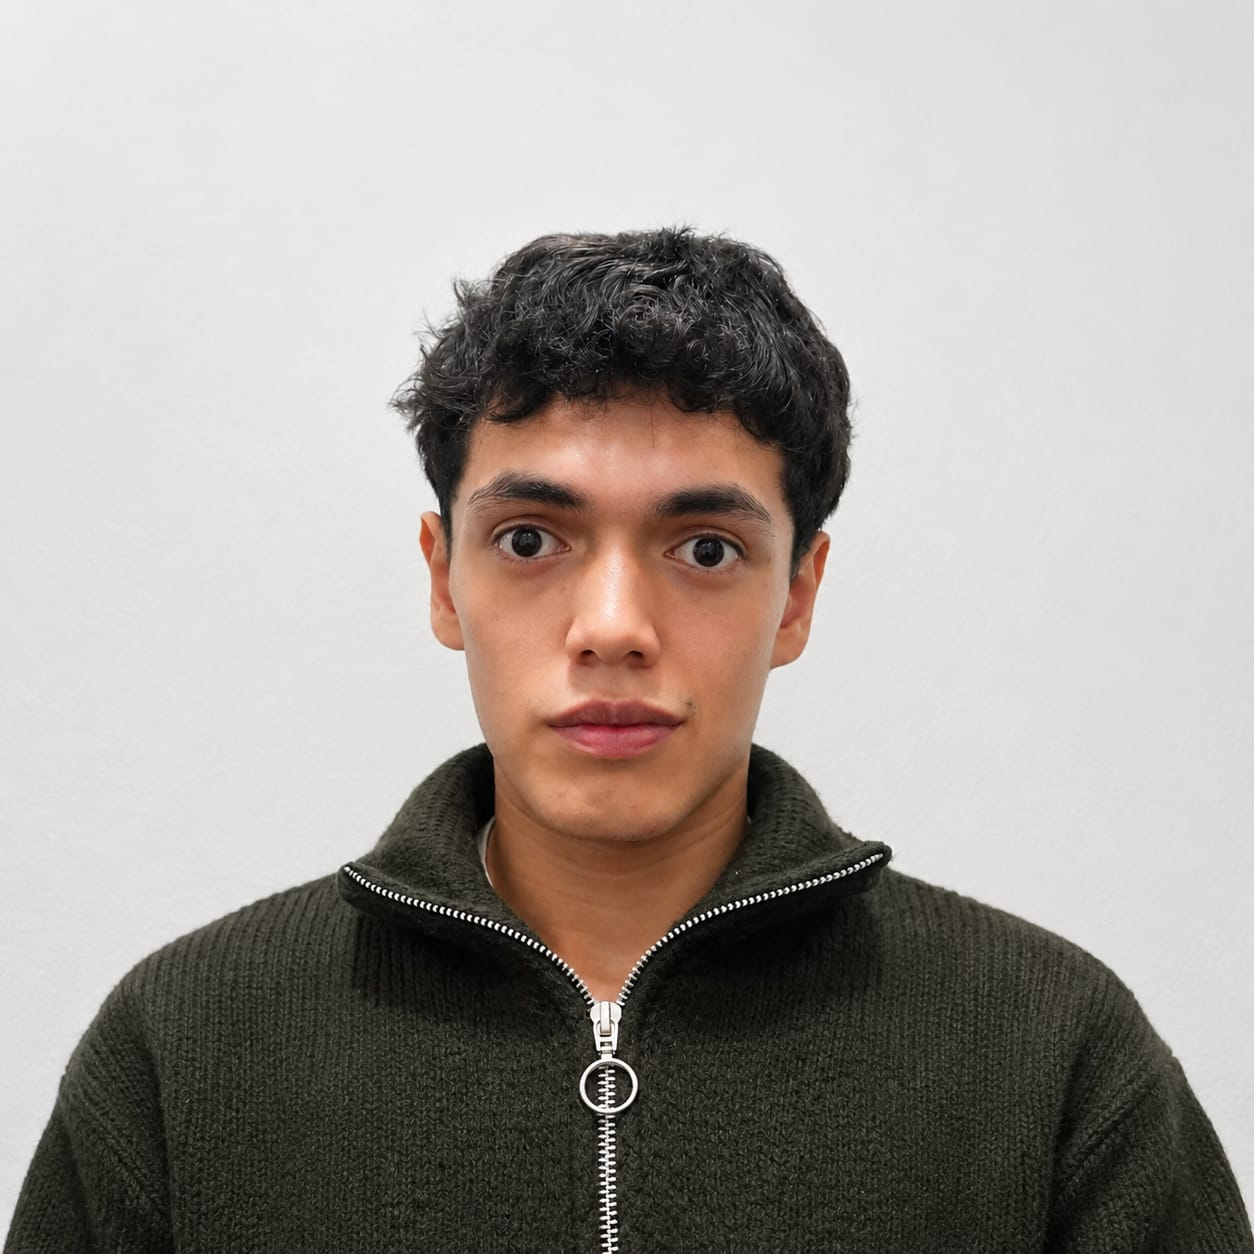
\includegraphics[width=3cm]{foto.jpg}};
\end{tikzpicture}
\end{center}
\vspace{6pt}

\sidetitle{Contacto}
\contact{\faPhone}{\href{https://wa.me/50239688410}{+502 3968-8410}}
\contact{\faEnvelope}{\href{mailto:madcarranzaosorio@gmail.com}{madcarranzaosorio@gmail.com}}
\contact{\faLinkedin}{\href{https://www.linkedin.com/in/miguel-angel-david-co-3585142a2/}{Miguel Ángel David Co}}
\contact{\faGithub}{\href{https://github.com/MADCO-py}{github.com/MADCO-py}}
\contact{\faGlobe}{\href{https://madco-py.github.io/CV-MIGUEL_CARRANZA/}{Portafolio en línea}}

\sidetitle{Datos personales}
\contact{\faUser}{20 años}
\contact{\faMapMarker*}{Zona 10, Guatemala}
\contact{\faCar}{Vehículo propio}
\contact{\faFile*}{NIT activo}

\sidetitle{Habilidades técnicas}
\skillgroup{Frontend}{HTML5, CSS3, JavaScript, TypeScript, React, Vite}
\skillgroup{Backend y lenguajes}{Node.js, Express, Python, Java, Kotlin, C / C++}
\skillgroup{Bases de datos}{PostgreSQL, Neo4J}
\skillgroup{Nube y despliegue}{Docker, Railway, Cloudflare R2, GitHub Pages}
\skillgroup{Herramientas}{Git, Linux, VS Code, Android Studio, Jetpack Compose, Jira}
\skillgroup{Hardware e IoT}{Arduino, ESP32, sensores, sistemas embebidos}

\sidetitle{Idiomas}
\contact{\faComment}{Español — 100\,\%}
\contact{\faComment}{Inglés — 80\,\%}

\sidetitle{Metodología}
{\fontsize{8.5}{11}\selectfont Trabajo ágil por sprints con gestión en Jira; código limpio y mantenible.}\par

\sidetitle{Áreas de interés}
{\fontsize{8.5}{11}\selectfont Ciberseguridad · Inteligencia artificial · Desarrollo web · Apps móviles · Sistemas y hardware · Backend y APIs}\par
\end{minipage}%
\hspace*{18pt}\hspace*{24pt}%
% ============================================================
%  COLUMNA PRINCIPAL
% ============================================================
\begin{minipage}[t][0.97\paperheight][t]{\dimexpr0.665\paperwidth-52pt\relax}
\vspace{26pt}

{\color{ink}\fontsize{30}{32}\selectfont\bfseries Miguel Carranza}\par
\vspace{5pt}
{\color{accent}\fontsize{11.5}{14}\selectfont\bfseries Desarrollador Full Stack}%
{\color{muted}\fontsize{11.5}{14}\selectfont\ \ ·\ \ Estudiante de Ingeniería en Computación}\par
\vspace{8pt}
Construyo software funcional, optimizado y mantenible: desde interfaces modernas hasta sistemas backend con bases de datos relacionales y de grafos, contenedores Docker y programación de microcontroladores. Estudiante de tercer año en la Universidad del Valle de Guatemala, con proyectos vendidos y en producción para clientes reales.\par

\maintitle{Experiencia}
\job{Desarrollador de software freelance}{Llantas Ávila — FleetControl}{Abr. 2026 · 30 h}
\begin{itemize}
  \item Desarrollé y entregué un sistema web de gestión de flota de camiones que resuelve un problema real: identificar qué piloto recibió una multa en un día determinado.
  \item 9 pilotos registrados con foto, fecha e historial de mantenimiento por vehículo; acceso con usuario y contraseña y registro vinculado por código QR.
  \item React, Node.js + Express y PostgreSQL; en producción en Railway con Docker y fotos en Cloudflare R2.
\end{itemize}
\vspace{5pt}
\job{Guía educativo}{Museo de los Niños de Guatemala}{Abr. 2025 – Oct. 2025}
\begin{itemize}
  \item Atención a niños y padres, comunicación efectiva, creación de contenido educativo digital y actividades dinámicas.
\end{itemize}
\vspace{5pt}
\job{Dependiente de tienda}{Bershka — Oakland Mall}{Nov. 2022 – Ene. 2023}
\begin{itemize}
  \item Servicio al cliente, apoyo en caja en horas de alta afluencia, control básico de inventario y organización de tienda.
\end{itemize}

\maintitle{Proyectos freelance vendidos}
\job{Los Skeepers — sitio oficial de banda}{\href{https://www.losskeepers.com/}{losskeepers.com} · dominio propio}{}
\begin{itemize}
  \item Interacción con fans y recolección de datos: analíticas anónimas, juegos con ranking mensual y validación anti-trampa, suscriptores y contenido editable desde un panel.
  \item Panel de administración privado con login (bcrypt, sesiones, límite de intentos) hecho en React + Vite + Recharts.
  \item Node.js + Express, PostgreSQL, Docker y Railway; exportación a Excel y tareas automáticas diarias.
\end{itemize}
\vspace{5pt}
\job{The Sunset Sessions — sitio de evento}{\href{https://madco-py.github.io/The-Sunset-Sessions/}{madco-py.github.io/The-Sunset-Sessions}}{}
\begin{itemize}
  \item Venta de entradas por WhatsApp, artistas por revelar, cuenta regresiva y marcas aliadas; React + htm sin compilación, en GitHub Pages.
\end{itemize}

\maintitle{Otros proyectos}
\begin{itemize}
  \item \textbf{\color{ink}SecureGate} — control de accesos con lectura de DPI y placas (Google Cloud Vision), React, Node.js, PostgreSQL y Docker.
  \item \textbf{\color{ink}MentorHub} — conecta 7 tutores universitarios con 20 estudiantes; React + Vite.
  \item \textbf{\color{ink}Sitios para emprendedores y artistas} — Walter Mazariegos, Nalú Korean Food, March Jewelry y Marce Juárez.
\end{itemize}

\maintitle{Educación}
\job{Ingeniería en Ciencias de la Computación y TI}{Universidad del Valle de Guatemala}{2023 – presente}
{\fontsize{8.8}{11.5}\selectfont Tercer año. Algoritmos, estructuras de datos, bases de datos, sistemas operativos y desarrollo de software.}\par
\vspace{6pt}
\job{Bachillerato en Ciencias y Letras, orientación en Computación}{Colegio Salesiano Don Bosco}{2020 – 2022}
{\fontsize{8.8}{11.5}\selectfont Graduado \textbf{Cum Laude}.}\par

\maintitle{Certificaciones}
\begin{itemize}
  \item \textbf{\color{ink}Creación de Páginas Web — HTML, CSS, JavaScript} · INTECAP, nivel intermedio.
  \item \textbf{\color{ink}HCI — Interacción Humano-Computadora} · Universidad del Valle de Guatemala.
  \item \textbf{\color{ink}Ética en Investigación con Sujetos Humanos} · UVG — CCSS, 8 h · 7 de mayo de 2026.
\end{itemize}
\end{minipage}

\end{document}
